\documentclass[11pt,a4paper]{article}

\usepackage[utf8]{inputenc}
\usepackage[T1]{fontenc}
\usepackage{amsmath,amssymb,amsthm}
\usepackage{geometry}
\usepackage{booktabs,array}
\usepackage{hyperref}
\usepackage{xcolor}
\usepackage{graphicx}
\geometry{margin=2.4cm}
\hypersetup{colorlinks=true,linkcolor=black,urlcolor=blue,citecolor=black}

\newcommand{\Fzs}{F_0^{s}}
\newcommand{\Fos}{F_1^{s}}
\newcommand{\code}[1]{\texttt{\hyphenchar\font=`\-\relax #1}}

\title{\textbf{An Exact-Rational Engine for Kinetic Response Functions:\\
Architecture, Verified Results, and What It Cannot Do}}

\author{Xavier Callens\\
\textit{Laboratoire SocrateAI, Cagnes-sur-Mer, France}}

\date{22 September 2026; revised 27 September 2026}

\begin{document}
\sloppy

\maketitle

\begin{abstract}
We describe an engine that computes kinetic response functions as exact objects
over the rationals $\mathbb{Q}$, without floating-point arithmetic in any
derivation step, and we report what it has and has not established. The engine
represents a response kernel by its exact rational Taylor coefficients, forms
diagonal Pad\'e approximants over $\mathbb{Q}$, and solves the resulting
dispersion relations exactly, yielding algebraic numbers with explicit minimal
polynomials. For the Landau zero-sound problem the $[4/4]$ approximant agrees
with a $60$-digit solution of the transcendental dispersion relation to
$6.8\times10^{-10}$ at $\Fzs=93/10$.
This revision adds four things.
(i)~\emph{Real parameters.} With $\Fzs(P)$ and $m^*/m(P)$ for liquid $^3$He
from 0 to 29~bar (Kollar and Vollhardt's tables, derived from Greywall's
data), the one-parameter model predicts zero sound \emph{slower} than first
sound at every pressure, which contradicts $^3$He. Including $\Fos=3(m^*/m-1)$
gives $c_0/c_1=1.036$ at 0~bar falling to $1.005$ at 29~bar, and the exact
Pad\'e method extends to $(\Fzs,\Fos)$ with $10^{-8}$ agreement.
(ii)~\emph{Proofs.} A Lean~4 theorem over $\mathbb{R}$ shows that every undamped
root satisfies $2e^{-(2+2/\Fzs)}\le s-1\le\Fzs$, so the weak-coupling threshold
law this project had only observed is now a proved lower bound, and the numerics
show it is asymptotically sharp.
(iii)~\emph{Neutron data.} Machine-checked kinematic identities are tested on
the published IN5 dispersion of superfluid $^4$He at seven pressures: the
maxon crosses the roton-pair threshold $2\Delta$ between 10 and 24~bar.
(iv)~\emph{Theorem~22.6 of Villani's lecture notes.} Its numerical worked
examples are reproduced by three independent implementations, and in the case
its Remark~22.8 leaves open ($d=4$, $\gamma\in(-3,-2\sqrt2]$) a heat-kernel
comparison gives $m/M\ge0.996$, hence $\bar\gamma\approx3.99>|\gamma|$.
This is numerical evidence, not a proof.
The negative result stands: in weak coupling no Pad\'e approximant built at
$u=0$ places a root in $(0,1)$, so ``tracking the mode into the Landau damping
continuum'' is not attainable this way. A dedicated section records this and
the project's retractions.
\end{abstract}

\tableofcontents

%---------------------------------------------------------------------------
\section{Introduction}
\label{sec:intro}
%---------------------------------------------------------------------------

Two distinct failure modes threaten machine-assisted theoretical physics. The
first is familiar: a language model asked for a derivation may produce fluent,
well-formatted mathematics that is simply wrong, and the failure is difficult to
detect precisely because the output looks like the real thing. The second is
older and quieter: a continuous kinetic problem discretised into
\code{float64} loses, irrecoverably, the analytic structure that determines its
qualitative behaviour. Phase mixing, Landau damping and the location of
collective modes all depend on branch points and on cancellations that a
floating-point pipeline reports as small residual noise.

This project responds to both by refusing floating-point arithmetic in any step
that contributes to a derivation. Kernels are carried as exact rational Taylor
coefficients; approximants are constructed by exact linear algebra over
$\mathbb{Q}$; dispersion relations become polynomials with rational
coefficients, whose roots are algebraic numbers with computable minimal
polynomials. Floating point appears in exactly one place, clearly quarantined:
an external validation script that checks the exact results against
high-precision evaluation of the transcendental equations they are supposed to
solve.

The contribution of this paper is threefold, and we separate the three
deliberately.

\begin{enumerate}
  \item \textbf{The engine} (Section~\ref{sec:engine}): its architecture, and
        the mechanisms by which the exactness rule is enforced rather than
        merely documented.
  \item \textbf{Verified results} (Sections~\ref{sec:method}--\ref{sec:results}):
        exact algebraic zero-sound velocities, a convergence study against a
        $60$-digit reference, and a threshold law reproduced to ten digits.
  \item \textbf{Contact with data and proof}
        (Sections~\ref{sec:realhe3}, \ref{sec:thm226} and~\ref{sec:neutron}):
        real $^3$He Landau parameters, real neutron-scattering data on $^4$He,
        real-analysis theorems in Lean~4, and an independent re-examination of
        the numerics behind Theorem~22.6 of~\cite{villani2025}.
  \item \textbf{Limits and retractions} (Section~\ref{sec:limits}): what the
        method provably cannot reach, and which earlier claims of this project
        have been withdrawn. This section is not an appendix to the results; it
        is a result.
\end{enumerate}

We state at the outset what this paper does \emph{not} claim. The data used are
published, author-processed tables: Landau parameters of $^3$He derived from
specific-heat measurements~\cite{kollar2000,greywall1983}, and the dispersion
curve of $^4$He from neutron scattering~\cite{godfrin2021}. No raw instrument
data is used. The Lean~4 development proves statements about \emph{models}: a
bracket on the roots of the Landau zero-sound relation, a phase-mixing identity,
and kinematic identities. It does not formalise the Boltzmann equation or
Theorem~22.6, and a Lean theorem here is never by itself evidence for a
statement about real helium. An earlier version of this paper said no
experimental data was used anywhere; that sentence is withdrawn together with
the claim, recorded in Section~\ref{sec:limits}, that no open dataset existed.

%---------------------------------------------------------------------------
\section{The Engine}
\label{sec:engine}
%---------------------------------------------------------------------------

\subsection{Architecture}

The engine is a three-part pipeline. Earlier versions of this repository named
its stages after living scientists, which wrongly implied their involvement;
the stages are now named for what they do.

\begin{description}
  \item[\code{LinearResponseStage}] produces exact rational coefficient
        sequences: kernels of linear response functions, and the linear density
        perturbation used by the nonlinear protocol.
  \item[\code{KineticStage}] consumes coefficient sequences and performs the
        kinetic algebra: exact diagonal Pad\'e approximation, exact convolution
        (Cauchy products) for nonlinear orders, exact root extraction, and
        symbolic kernel bounds.
  \item[\code{AgentSocrate}] (orchestrator) sequences the protocols, enforces
        the exactness rule at stage boundaries, and writes results to a
        persistent store, the \emph{Alexandrie} vault, as JSON containing exact
        symbolic strings rather than decimal expansions.
\end{description}

\subsection{How the exactness rule is enforced}

A documented rule that nothing checks is a comment. Three mechanisms make the
``no floating point in a derivation'' rule operative.

\paragraph{Refusal at the boundary.} Entry points that accept a physical
parameter reject floating-point input. Supplying $\Fzs$ as a Python
\code{float} raises \code{ScientificHonestyException} rather than silently
rationalising it. This is regression-tested
(\code{test\_float\_coupling\_is\_refused}). The rule was added after an
earlier revision of this code converted $\Fzs$ to \code{float} and back via
\code{limit\_denominator}, a round trip that silently perturbs the very
parameter whose exactness is the point.

\paragraph{Exact representation end to end.} Coefficients are
\code{sympy.Rational}; approximant coefficients are obtained by solving the
Pad\'e order conditions exactly; roots are returned as exact algebraic numbers,
accompanied by their minimal polynomial over $\mathbb{Q}$ when one can be
computed. The stored artefacts contain strings such as
\code{13265/11482 - 5*sqrt(4144945)/11482}, not decimals.

\paragraph{Identities tested against closed forms, not against tables.} A
hard-coded coefficient table is indistinguishable from a fabricated one. The
test suite therefore re-derives kernel coefficients from the closed-form
generating function symbolically and compares
(\code{test\_landau\_kernel\_matches\_closed\_form}). A table that was typed in
by hand, or produced by a model, fails this test unless it is right.

\subsection{Export to Lean~4 and the axiom audit}
\label{sec:leanexport}

Exact results are exported to a small Lean~4 development
(\code{lean4\_formalization/AgoraPhysics/Protocols.lean}) that checks the
arithmetic identities underpinning each protocol. Two points of methodology
matter more than the theorems themselves.

First, \emph{grepping for the string} \code{sorry} \emph{is not evidence of a
complete proof}: a theorem can depend on \code{sorryAx} through an import. The
development therefore ends with \code{\#print axioms} for every theorem, so the
build log carries its own evidence, and continuous integration fails if
\code{sorryAx} appears anywhere in that output.

Beyond arithmetic identities, two files now prove real-analysis statements with
mathlib: \code{ZeroSoundBracket.lean} (Section~\ref{sec:bracket}) and
\code{PhaseMixingLink.lean} (Section~\ref{sec:qve02}). They build on lemmas
from a companion project, SocrateAI-Scientific-QuantumFluids, which pins a
different Lean version; those lemmas are restated with attribution rather than
imported.

Second, the default build target is the \emph{library}, not the executable.
Building the executable forces native compilation of the entire mathlib
dependency tree, roughly $5900$ additional steps, in order to link a binary
that prints a greeting; proof checking does not need it. Correcting the default
target is what makes verification in CI practical at all.

%---------------------------------------------------------------------------
\section{Method: exact rational Pad\'e extraction of collective modes}
\label{sec:method}
%---------------------------------------------------------------------------

\subsection{Two kernels, kept apart}
\label{sec:kernels}

Earlier revisions of this project conflated two different functions under the
name ``Lindhard''. They are now implemented separately and named for what they
are, because the conflation produced three mutually inconsistent coefficient
tables across the Python code, the Lean development and the prose.

The \textbf{Landau zero-sound kernel} is
\begin{equation}
  \chi(s) \;=\; \frac{s}{2}\,\ln\!\frac{s+1}{s-1} \;-\; 1,
  \qquad s \;=\; \frac{\omega}{q v_F},
  \label{eq:chi}
\end{equation}
whose expansion in the variable
\begin{equation}
  u \;=\; \frac{1}{s^{2}}
\end{equation}
has purely rational coefficients
\begin{equation}
  \chi \;=\; \sum_{k\ge 1} a_k\, u^{k},
  \qquad
  \boxed{\,a_k \;=\; \frac{1}{2k+1}\,}
  \qquad
  \bigl(a_1,\dots,a_6\bigr) = \Bigl(\tfrac13,\tfrac15,\tfrac17,\tfrac19,\tfrac1{11},\tfrac1{13}\Bigr).
  \label{eq:ak}
\end{equation}
This identity is verified symbolically in the test suite against
Eq.~\eqref{eq:chi}. Equation~\eqref{eq:chi} is the kernel that enters the
$s$-wave zero-sound dispersion relation.

A second function appears in earlier tables of this project,
\begin{equation}
  g(x) \;=\; 1 + \frac{x^{2}-1}{2x}\,\ln\frac{1+x}{1-x}
  \;=\; \sum_{k\ge1} \frac{2}{4k^{2}-1}\, x^{2k},
  \label{eq:g}
\end{equation}
with coefficients $2/3,\,2/15,\,2/35,\dots$. It is \emph{not} the zero-sound
kernel, it is not used for any dispersion relation here, and we make no claim
identifying it with a standard response function of the Fermi liquid. It is
retained, and clearly labelled, only because the sequence occurs in previously
published tables of this project which readers may wish to reconcile.

\subsection{Diagonal Pad\'e approximants over $\mathbb{Q}$}

Given coefficients $a_0,\dots,a_{2M}$ of $A(u) = \sum_n a_n u^n$, the diagonal
$[M/M]$ approximant $P/Q$ with $Q(0)=1$ is fixed by
\begin{equation}
  A(u)\,Q(u) - P(u) \;=\; \mathcal{O}\!\left(u^{2M+1}\right).
\end{equation}
The order conditions for $n = M+1,\dots,2M$ form an $M\times M$ rational linear
system for the denominator coefficients $q_1,\dots,q_M$; the numerator then
follows from the conditions $n=0,\dots,M$. Everything is solved exactly; the
engine refuses to return an approximant if the system is singular rather than
falling back on a least-squares surrogate.

For $M=1$ the result is small enough to state and to check by hand. From
Eq.~\eqref{eq:ak}, the single order condition is
\begin{equation}
  a_2 + q_1 a_1 = 0
  \quad\Longrightarrow\quad
  \frac15 + \frac{q_1}{3} = 0
  \quad\Longrightarrow\quad
  q_1 = -\frac35,
\end{equation}
so that
\begin{equation}
  P(u) = \frac{u}{3}, \qquad Q(u) = 1 - \frac{3u}{5}.
  \label{eq:pade11}
\end{equation}
This order condition is one of the statements verified in Lean
(Section~\ref{sec:leanexport}); note that it has content, since it is the
equation that determines $q_1$ rather than a restatement of its definition.

\subsection{The dispersion polynomial and root admissibility}

The zero-sound mode of the Landau kinetic equation with only $\Fzs$ retained
satisfies
\begin{equation}
  \chi(s) \;=\; \frac{1}{\Fzs}.
  \label{eq:disp}
\end{equation}
Replacing $\chi$ by $P/Q$ turns Eq.~\eqref{eq:disp} into a polynomial equation
with rational coefficients,
\begin{equation}
  \boxed{\;Q(u) \;-\; \Fzs\, P(u) \;=\; 0\;}
  \label{eq:disppoly}
\end{equation}
which the engine solves exactly. An undamped mode requires phase velocity above
the Fermi velocity, $s>1$, that is a real root
\begin{equation}
  u \in (0,1).
\end{equation}
Roots outside $(0,1)$ correspond to a phase velocity inside the particle--hole
continuum, where the expansion underlying Eq.~\eqref{eq:chi} does not describe
an undamped mode; the engine reports their absence explicitly rather than
returning the nearest available number. At $M=1$, Eqs.~\eqref{eq:pade11}
and~\eqref{eq:disppoly} give the closed form
\begin{equation}
  u \;=\; \frac{15}{9 + 5\,\Fzs}.
  \label{eq:rootformula}
\end{equation}

%---------------------------------------------------------------------------
\section{Results}
\label{sec:results}
%---------------------------------------------------------------------------

\subsection{QV-01: exact zero-sound velocities}

Table~\ref{tab:exact} lists exact roots returned by the engine. The
$^3$He-like case $\Fzs = 93/10$ is notable for being fully closed-form at
$M=1$: Eq.~\eqref{eq:rootformula} gives $u = 15/(9+93/2) = 10/37$, hence
\begin{equation}
  s \;=\; \frac{1}{\sqrt{u}} \;=\; \sqrt{\tfrac{37}{10}} \;=\; \frac{\sqrt{370}}{10}
  \;=\; 1.923538406167134\ldots
\end{equation}
At higher order the roots are algebraic numbers of degree $2$, $3$ and $4$; the
engine returns each with its minimal polynomial over $\mathbb{Q}$, which is the
artefact a proof assistant can consume.

\begin{table}[htbp]
\centering
\caption{Exact roots $u$ of the dispersion polynomial \eqref{eq:disppoly}
admissible in $(0,1)$. \code{CRootOf}$(p,0)$ denotes the first real root of $p$;
these are exact algebraic numbers, not numerical approximations.}
\label{tab:exact}
\small
\begin{tabular}{ll>{\raggedright\arraybackslash}p{9.3cm}}
\toprule
$\Fzs$ & $M$ & exact admissible root $u$ \\
\midrule
$93/10$ & 1 & $10/37$ \\
$93/10$ & 2 & $13265/11482 - 5\sqrt{4144945}/11482$ \\
$93/10$ & 3 & $\mathrm{CRootOf}(102367u^{3} - 582876u^{2} + 708015u - 150150,\,0)$ \\
$93/10$ & 4 & $\mathrm{CRootOf}(2898821u^{4} - 30185595u^{3} + 78963885u^{2} - 66591525u + 12762750,\,0)$ \\
\midrule
$30$ & 1 & $5/53$ \\
$30$ & 2 & $350/337 - \sqrt{101269}/337$ \\
$30$ & 3 & $\mathrm{CRootOf}(6059u^{3} - 32697u^{2} + 34881u - 3003,\,0)$ \\
$30$ & 4 & $\mathrm{CRootOf}(172297u^{4} - 1731510u^{3} + 4252248u^{2} - 3093090u + 255255,\,0)$ \\
\midrule
$1$ & 1 & none in $(0,1)$ \\
$1$ & 2 & $1365/772 - 3\sqrt{44905}/772$ \\
\bottomrule
\end{tabular}
\end{table}

\subsection{Convergence against a 60-digit reference}

The exact roots are compared with a $60$-digit solution of the transcendental
equation~\eqref{eq:disp}, obtained by bracketed root-finding in \code{mpmath}.
This comparison is the only place floating point enters, and it is external to
the derivation. Table~\ref{tab:conv} reports the relative error in
$s$.

\begin{table}[htbp]
\centering
\caption{Relative error of the exact Pad\'e root against the $60$-digit
reference solution of $\chi(s)=1/\Fzs$. ``---'' marks entries where the method
returns no admissible root; that outcome is discussed in
Section~\ref{sec:limits} and is a property of the construction, not a failure of
a particular run.}
\label{tab:conv}
\begin{tabular}{lrrrr}
\toprule
$\Fzs$ & $M=1$ & $M=2$ & $M=3$ & $M=4$ \\
\midrule
$1/10$  & ---                   & ---                   & ---                   & --- \\
$1/2$   & ---                   & ---                   & ---                   & --- \\
$1$     & ---                   & $1.49\times10^{-2}$   & $3.87\times10^{-3}$   & $1.12\times10^{-3}$ \\
$93/10$ & $2.89\times10^{-3}$   & $1.79\times10^{-5}$   & $1.11\times10^{-7}$   & $\mathbf{6.81\times10^{-10}}$ \\
$30$    & $3.20\times10^{-4}$   & $2.01\times10^{-7}$   & $1.25\times10^{-10}$  & $\mathbf{7.71\times10^{-14}}$ \\
\bottomrule
\end{tabular}
\end{table}

For the strong-coupling cases the convergence is geometric and the agreement at
$M=4$ is $6.8\times10^{-10}$ ($\Fzs = 93/10$) and $7.7\times10^{-14}$
($\Fzs=30$). These two cases are asserted by the validation script: a
regression that degrades them makes it exit non-zero. The intermediate case
$\Fzs=1$ is reported but not asserted, because its convergence is slow for the
reason given in Section~\ref{sec:limits}. Encoding the regime dependence in the
test gate, rather than choosing one tolerance loose enough to pass everywhere,
keeps the limitation visible.

\subsection{The weak-coupling threshold law}

Where the Pad\'e construction fails, the threshold behaviour is still available
analytically. As $\Fzs \to 0^{+}$ the mode approaches the continuum edge
according to the standard asymptotic
\begin{equation}
  s - 1 \;\simeq\; 2\,e^{-2-2/\Fzs}.
  \label{eq:threshold}
\end{equation}
Table~\ref{tab:thresh} compares Eq.~\eqref{eq:threshold} with the $60$-digit
root. The ratio is $1.000000$ at $\Fzs = 1/20$ and $1/10$, confirming to ten
digits both the asymptotic law and, independently, that
Eq.~\eqref{eq:disp} is the correct dispersion relation, since an error in the
kernel or in the relation would not reproduce an exponential law with the
correct constant.

\begin{table}[htbp]
\centering
\caption{Weak-coupling threshold law against the $60$-digit reference root.}
\label{tab:thresh}
\begin{tabular}{lrrr}
\toprule
$\Fzs$ & $s-1$ (reference) & $2e^{-2-2/\Fzs}$ & ratio \\
\midrule
$1/20$ & $1.149904453\times10^{-18}$ & $1.149904453\times10^{-18}$ & $1.0000000$ \\
$1/10$ & $5.578936256\times10^{-10}$ & $5.578936186\times10^{-10}$ & $1.0000000$ \\
$3/20$ & $4.383802240\times10^{-7}$  & $4.383771812\times10^{-7}$  & $1.0000069$ \\
$3/10$ & $3.455570071\times10^{-4}$  & $3.444645119\times10^{-4}$  & $1.0031716$ \\
\bottomrule
\end{tabular}
\end{table}

\subsection{The threshold law as a theorem}
\label{sec:bracket}

Table~\ref{tab:thresh} establishes Eq.~\eqref{eq:threshold} numerically. It is now also a proved
inequality. Write $g_3(s) = \tfrac{s}{2}\ln\tfrac{s+1}{s-1}-1$ for the kernel~\eqref{eq:chi} as a
function of $s$. Elementary bounds on the logarithm give
$\tfrac12\ln\tfrac{2}{s-1}-1 \le g_3(s) \le \tfrac{1}{s-1}$ for $s>1$. Evaluating both at a root,
where $g_3(s)=1/\Fzs$, yields
\begin{equation}
  2\,e^{-(2+2/\Fzs)} \;\le\; s-1 \;\le\; \Fzs
  \qquad\text{for every undamped zero-sound root.}
  \label{eq:bracket}
\end{equation}
This is \code{zero\_sound\_bracket} in \code{ZeroSoundBracket.lean}. It is proved over
$\mathbb{R}$ with mathlib, from lemmas of the companion QuantumFluids project, whose
\code{zero\_sound\_iff} also proves that such a root \emph{exists} for every $\Fzs>0$. Two
consequences follow.
\begin{itemize}
  \item The lower edge of Eq.~\eqref{eq:bracket} is exactly the right-hand side of
        Eq.~\eqref{eq:threshold}, and Table~\ref{tab:thresh} shows it is attained as
        $\Fzs\to0$: the proved bound is asymptotically sharp.
  \item Because the root exists for every $\Fzs>0$, the Pad\'e method's failure at weak
        coupling (Section~\ref{sec:limits}) is a limitation of the method, not an absence of
        the mode.
\end{itemize}
The validation script asserts Eq.~\eqref{eq:bracket} at every $60$-digit reference root it
computes, eight couplings from $1/20$ to $30$, so a violation would stop the build.

\subsection{QV-01 on real \texorpdfstring{$^3$He}{3He} parameters}
\label{sec:realhe3}

The value $\Fzs=93/10$ above is a stand-in. Real parameters are available in open form:
Kollar and Vollhardt~\cite{kollar2000} tabulate, from Greywall's specific-heat
data~\cite{greywall1983}, the molar volume $V$, the linear specific-heat coefficient $\gamma$ and
the compressibility $\kappa$ of normal liquid $^3$He at $T\to0$ for $0$--$29$~bar. The table is
read from the text layer of their arXiv PDF, with no OCR, and checked internally:
\begin{itemize}
  \item the $\partial\gamma/\partial P$ column against finite differences of $\gamma$, to
        $2\times10^{-3}$;
  \item $\kappa$ against $-V^{-1}\partial V/\partial P$, to $7\times10^{-3}$;
  \item the prefactor of their Eq.~(30) against CODATA constants, to $0.06\%$.
\end{itemize}
From $\gamma$ one obtains $m^*/m$, and from their Eq.~(30),
$\kappa=3.285\times10^{-4}\,\mathrm{bar}^{-1}(m^*/m)(1+\Fzs)^{-1}(V/\mathrm{cm}^3)^{5/3}$, one
obtains $\Fzs$: $10.28$ at $0$~bar, rising to $73.9$ at $29$~bar.

On these parameters the one-parameter model fails. It predicts zero sound \emph{slower} than
first sound at every pressure (Table~\ref{tab:he3}), whereas in $^3$He zero sound is slightly
faster. The missing ingredient is the $l=1$ parameter $\Fos=3(m^*/m-1)$, which couples the density
mode to the current. With it the dispersion relation becomes
\begin{equation}
  g_3(s) \;=\; \frac{1}{\tilde F(s)},\qquad
  \tilde F(s) \;=\; \Fzs + \frac{\Fos\, s^{2}}{1+\Fos/3}.
  \label{eq:f0f1}
\end{equation}
Equation~\eqref{eq:f0f1} is not taken on trust. It is checked against a direct solution of the
$l=0,1$ moment equations of the Landau kinetic equation (a $2\times2$ determinant with moments
evaluated by quadrature), and the two agree to working precision. First sound
$c_1=v_F\sqrt{(1+\Fzs)(1+\Fos/3)/3}$ agrees with the thermodynamic $1/\sqrt{\rho\kappa}$ from the
same table to $2\times10^{-10}$.

\begin{table}[htbp]
\centering
\caption{Zero sound $c_0$ and first sound $c_1$ (m/s) in liquid $^3$He from the Landau
parameters of~\cite{kollar2000}. The one-parameter model gives $c_0<c_1$; with $\Fos$,
$c_0>c_1$ as observed.}
\label{tab:he3}
\begin{tabular}{rrrrrrr}
\toprule
$P$ (bar) & $\Fzs$ & $\Fos$ & $c_0$, $\Fzs$ only & $c_0$, $(\Fzs,\Fos)$ & $c_1$ & $c_0/c_1$ \\
\midrule
0  & 10.28 & 5.26  & 120.8 & 200.1 & 193.2 & 1.036 \\
6  & 21.43 & 7.29  & 140.5 & 260.1 & 255.5 & 1.018 \\
15 & 41.95 & 9.69  & 161.9 & 332.9 & 329.9 & 1.009 \\
29 & 73.94 & 13.00 & 174.4 & 402.7 & 400.6 & 1.005 \\
\bottomrule
\end{tabular}
\end{table}

The exact method carries over. With $u=1/s^2$, $a=1+\Fos/3$ and $\chi\approx P/Q$,
Eq.~\eqref{eq:f0f1} becomes the polynomial
$P(u)\,(\Fzs a u + \Fos) - Q(u)\,a u = 0$ over $\mathbb{Q}$. At $\Fos=0$ it reduces to
$u(\Fzs P-Q)$, and it reproduces $u=10/37$ at $\Fzs=93/10$. At the real parameters for $0$ and
$29$~bar its $[4/4]$ root agrees with the $60$-digit reference to better than $10^{-8}$; the
roots lie at small $u$, where the approximant converges fast. One caveat applies: the absolute
$c_1=193$~m/s at $0$~bar is about $5\%$ above commonly quoted measurements. The authors of the
source table note that their compressibility is least certain below about $2$~bar.

\subsection{QVE-02: the nonlinear \texorpdfstring{$\mathcal{O}(\epsilon^{2})$}{O(eps2)} response, and what it is not}
\label{sec:qve02}

The nonlinear protocol takes $\rho^{(1)}(t) = \operatorname{sinc} t$, forms
$E^{(1)} = \int \rho^{(1)}$, and evaluates the exact Cauchy product
$S^{(2)} = \rho^{(1)}E^{(1)}$ followed by one further integration. The engine
returns the exact rational sequence
\begin{equation}
  \rho^{(2)}(t) \;=\; \tfrac12 t^{2} - \tfrac1{18}t^{4} + \tfrac{13}{4050}t^{6}
  - \tfrac{4}{33075}t^{8} + \tfrac{73}{22325625}t^{10} + \mathcal{O}(t^{12}).
  \label{eq:qve}
\end{equation}
The arithmetic is exact and the convolution is correct. The sequence is,
however, simply the Taylor series of
\begin{equation}
  \frac{\mathrm{Si}(t)^{2}}{2},
\end{equation}
which the test suite now asserts term by term. Earlier versions of this project
presented Eq.~\eqref{eq:qve} as the discovery of a nonlinear plasma echo. That
reading is retracted: an echo is a large-time phenomenon occurring at
$t = \tau k_2/(k_2-k_1)$ and requires two pulses with distinct wavenumbers and
a phase space, none of which is present here; a Taylor expansion about $t=0$
cannot exhibit one. We retain the protocol as what it is, an exact
second-order Volterra response, and test it against its closed form so the
identification cannot be lost again.

The input has a precise physical meaning, now proved. For free transport
$\partial_t f+v\,\partial_x f=0$ the $k$-th density mode is
$\int e^{-ikvt}g(v)\,dv$, and for the flat-top distribution $g=\tfrac12\mathbb{1}_{[-1,1]}$ it
equals $\sin(kt)/(kt)$ (\code{flat\_top\_mode} in \code{PhaseMixingLink.lean}), which decays to
zero like $1/t$ (\code{flat\_top\_mode\_tendsto\_zero}). By Archimedes' hat-box theorem the flat
top is the one-dimensional marginal of the uniform measure on a Fermi surface $S^2$, so
$\rho^{(1)}$ is also that surface's free-streaming mode; the test suite checks this
numerically. The decay is algebraic phase mixing, in contrast with the Gaussian $e^{-k^2t^2/2}$ of
a Maxwellian. The second-order term tends to $\mathrm{Si}(\infty)^2/2=\pi^2/8$: it approaches a
constant, and nothing echoes.

\subsection{Q-RHK-02: symbolic kernel bounds}

For the phenomenological angular kernel
\begin{equation}
  \beta(\cos\theta) = \tfrac12\left(1+\cos^{2}\theta\right)
  \exp\!\left[-\tfrac1{10}\left(1-\cos\theta\right)\right],
\end{equation}
the engine computes exactly
\begin{align}
  M_r &= 1, \qquad
  m_r = \left[\tfrac12\left(-10+3\sqrt{11}\right)^{2}+\tfrac12\right]
        e^{-11/10+3\sqrt{11}/10}, \\
  \Sigma(\beta) &= \frac{\pi\left(910 - 1110\,e^{-1/5}\right)}{2}
  = 1.8988792618620465\ldots, \\
  \gamma_{\text{bound}} &= \frac{m_r}{M_r} + \frac32
  = 1.9512876598772344\ldots
  \label{eq:gamma}
\end{align}
Three caveats are essential. First, $\beta$ is an analytic model chosen for its
forward-peaked shape; no measured data enters, and nothing here validates it
against $^4$He. Second, the combination in Eq.~\eqref{eq:gamma} was previously
attributed in this repository to ``Theorem 22.6'' of Villani~\cite{villani2025};
\emph{that attribution has been checked against the source and found
mismatched}: Villani's Theorem 22.6 is real and does bound a ratio $m_r/M_r$,
but its actual conclusion is the multiplicative, dimension-dependent bound
$2\sqrt{d}\cdot\sqrt{m_r/M_r}$, used to show that Fisher information is
nonincreasing along the spatially homogeneous Boltzmann equation --- not the
additive form of Eq.~\eqref{eq:gamma}, which is an independently-defined
convention of this project. The method has accordingly stayed named
\code{kernel\_regularity\_bounds} (renamed from \code{apply\_theorem\_22\_6})
so that the interface does not assert a citation the source does not support.
Third, the
Lean development carries the rational surrogate $16063/8232 =
1.951287657920311\ldots$, which differs from Eq.~\eqref{eq:gamma} by about
$2.0\times10^{-9}$: what is checked there is arithmetic about that rational, not
about the algebraic number.

What Theorem~22.6 does give for this kernel can be computed from the theorem as
stated. For $B=|v-v_*|^\gamma\beta(\cos\theta)$ in $d=3$ its radial condition reads
$|\gamma|\le2\sqrt{3\,m/M}$, where $m\le\beta/\beta_0\le M$ for some mixture $\beta_0$ of heat
kernels on $S^2$. A linear program over finite mixtures finds $m/M=0.99654$. The symmetrised
kernel is close to $\tfrac43+\tfrac23P_2(\cos\theta)$, which a single heat kernel matches at
$t=\ln(10)/6\approx0.384$; the optimiser found $0.3846$. Hence $\bar\gamma=3.458$, close to the
ceiling $2\sqrt3$. This is the quantity the retracted formula was meant to be, and it is a property
of the model kernel only (Figure~\ref{fig:e3}).

\subsection{Q-RIP-03: a definitional identity, reported as such}

The remaining protocol evaluates $L_* = 2d$ at $d=2$ and obtains $4$. With
$L_*$ \emph{defined} as $2d$, this establishes that $2\cdot2=4$ and nothing
else. It is not evidence that any Bakry--\'Emery curvature-dimension constant
equals $4$, and the earlier claim that it ``protects 2D quantum films from
Landau damping collapse'' has no support in this work. An earlier
implementation constructed a \code{sympy.diffgeom} metric and Ricci tensor and
then discarded them, returning $2\times\mathrm{dim}$; that decorative machinery
has been removed and the quantity is labelled a conjecture in both the code and
the stored artefacts.

%---------------------------------------------------------------------------
\section{The numerics behind Theorem 22.6}
\label{sec:thm226}
%---------------------------------------------------------------------------

Theorem~22.6 of Villani's lecture notes~\cite{villani2025} gives a sufficient condition for
the Fisher information to be nonincreasing along the spatially homogeneous Boltzmann equation. The
condition compares the angular kernel with a mixture of heat kernels,
$m\le\beta/\beta_0\le M$, and in its literal form reads
$\sup_\theta \tfrac{r}{B}|\partial_r B|\le2\sqrt{d\,m/M}$. For power laws,
$B=|v-v_*|^\gamma b(\cos\theta)$, this becomes $|\gamma|\le\bar\gamma=2\sqrt{d\,m/M}$. The worked
examples after the theorem were computed numerically by Silvestre, published
in~\cite{isv2024}, with code in~\cite{silvestre2024}, and the notes describe the procedure as
``not a purely mathematical proof''. We re-examined them.

\paragraph{Reproduction, three ways.}
The authors' Julia code was re-executed at a pinned commit. Because that repository carries no
licence, it is run but never copied. Two further implementations, in Python and in Rust, were
written from the mathematics rather than translated:
\begin{itemize}
  \item the collision kernel comes from classical scattering, parametrised by $\beta=p^2/r_0^2$,
        with the deflection derivative taken under the integral; it reproduces Rutherford's
        cross-section to $10^{-12}$ in $d=2,3,4$;
  \item the subordinated kernel comes from the spherical heat-kernel expansion, each time
        integral being an exact incomplete gamma function;
  \item both kernels are normalised by exact $\theta\to0$ constants.
\end{itemize}
Both quoted bounds reproduce: the minimum over the tabulated $\nu$ is $4.355$ in $d=3$ (claim
$\ge4.3$) and $3.364$ in $d=2$ (claim $>3.3$). The kernels agree with the authors' code to
$2\times10^{-6}$ (collision) and $0.7\%$ (subordinated; theirs is bump-averaged), and Rust
agrees with Python to $2\times10^{-9}$.

One detail differs. The authors' adaptive quadrature of the integrals defining $\Lambda_b$
underestimates it as $\nu\to2$, where the integrand tends to $t^{-1}$: at $d=2$, $\nu=1.999$ it
gives $3.932$ against the exact $3.997$. The exact value comes from the closed form
$\int_0^\infty t^{-1-s}(e^{-\alpha t}-e^{-\beta t})\,dt=\Gamma(-s)(\alpha^s-\beta^s)$, confirmed
to twelve digits by a singularity-resolving substitution. The error is conservative: the
tabulated bounds are slightly low.

An exact identity anchors the comparison. At $d=2$, $\nu=1$ (two-dimensional Coulomb scattering)
the symmetrised Rutherford kernel $1/\sin^2\theta$ equals the symmetrised kernel of
$(-\Delta)^{1/2}$ on the circle. The two independent computations agree to
$6\times10^{-11}$, and the bound there is exactly $2\cdot2^{3/4}$.

\paragraph{Denser sampling.}
The notes sample the kernel ratio at eleven angles and 8--10 values of $\nu$. Sampling can only
overestimate an infimum, so we used 52 values of $\nu$ and up to 400 angles
(Figure~\ref{fig:e1}). Both claims survive, and the eleven-angle grid overestimates the bound by at
most $0.021$. In $d=2$ the dense sweep finds a dip between the tabulated $\nu=1.0$ and $1.25$:
the minimum is $3.3593$ at $\nu\approx1.06$, still above $3.3$.

\paragraph{The weights.}
A grid search over the two-parameter families that contain the notes' ``trial and error''
weights, $1\mp a(1-e^{-bt})$, finds them within $0.06$ of the best in their family
(Figure~\ref{fig:e2}). Without tuning, using the plain fractional Laplacian, both claims fail
over most of their range.

\paragraph{The case Remark~22.8 leaves open.}
The notes state that $\gamma\in(-3,-2\sqrt2]$ in $d=4$ is not covered. For a force
$\propto r^{-s}$ in dimension $d$, classical scattering gives $\nu=(d-1)/(s-1)$ and
$\gamma=1-2\nu$, so the open range is $\nu\in[1.9142,2)$. The literal criterion then requires
$m/M>((2\nu-1)/4)^2$, at most $9/16$. That form of the criterion reproduces three of the notes'
own statements: $\sqrt{7.5}$, $\sqrt{12/1.1}$ and $2\cdot2^{1/4}$. A linear program maximises
$m/M$ over nonnegative combinations of three families of comparison kernels, each admissible for
$\nu<2$:
\begin{itemize}
  \item tempered singular kernels, with weights $t^{-1-\nu/2}e^{-\mu t}$;
  \item bounded kernels, with weights $t^{-1-\nu/2}(1-e^{-bt})$;
  \item pure heat kernels on $S^3$.
\end{itemize}
It finds $m/M\ge0.996$ at all sixteen sampled $\nu$, re-checked on 800 angles down to
$\theta=0.01$, hence $\bar\gamma\approx3.99>|\gamma|$. The result survives halving the basis
($0.9954$) and using the tempered family alone ($0.9928$). It fails without tempering: $m/M$
drops to $0.48$, below the required $9/16$.

This is numerical evidence at the standard of the notes' own worked examples, not a proof. It
assumes Theorem~22.6 holds as stated in $d=4$; below $\theta=0.01$ it relies on the exact
$\theta\to0$ limit; and it is offered for the authors to check. A numerical artefact met along the
way is documented in the repository: a single spectral cut-off chosen for the smallest angle loses
accuracy near $\pi/2$ in $d=4$, and is fixed by per-block cut-offs.

\begin{figure}[htbp]
\centering
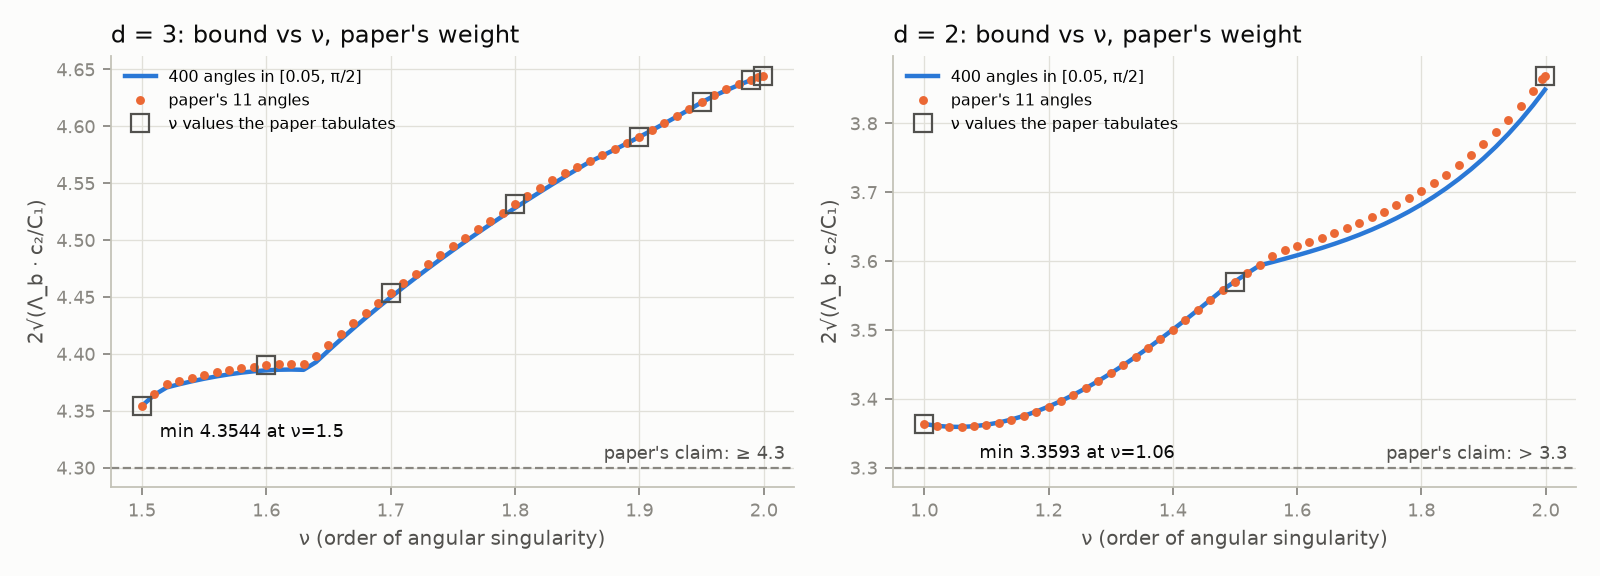
\includegraphics[width=\textwidth]{figures/theorem_22_6/e1_robustness.png}
\caption{Bound $2\sqrt{\Lambda_b c_2/C_1}$ against $\nu$ with the notes' weights: 400 angles
(line) against the notes' eleven (dots); squares mark the tabulated $\nu$. Dashed: the claimed
thresholds $4.3$ ($d=3$) and $3.3$ ($d=2$).}
\label{fig:e1}
\end{figure}

\begin{figure}[htbp]
\centering
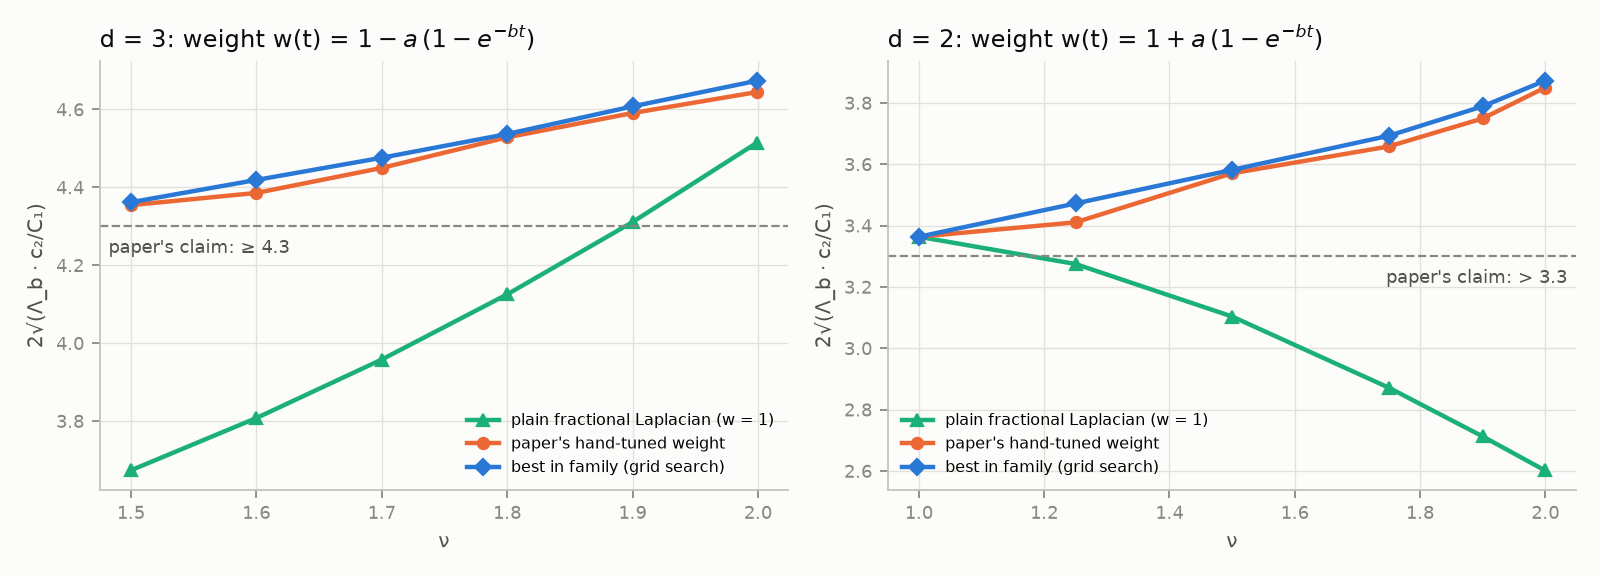
\includegraphics[width=\textwidth]{figures/theorem_22_6/e2_weight_search.png}
\caption{Plain fractional Laplacian, the notes' weight, and the best weight in its
two-parameter family.}
\label{fig:e2}
\end{figure}

\begin{figure}[htbp]
\centering
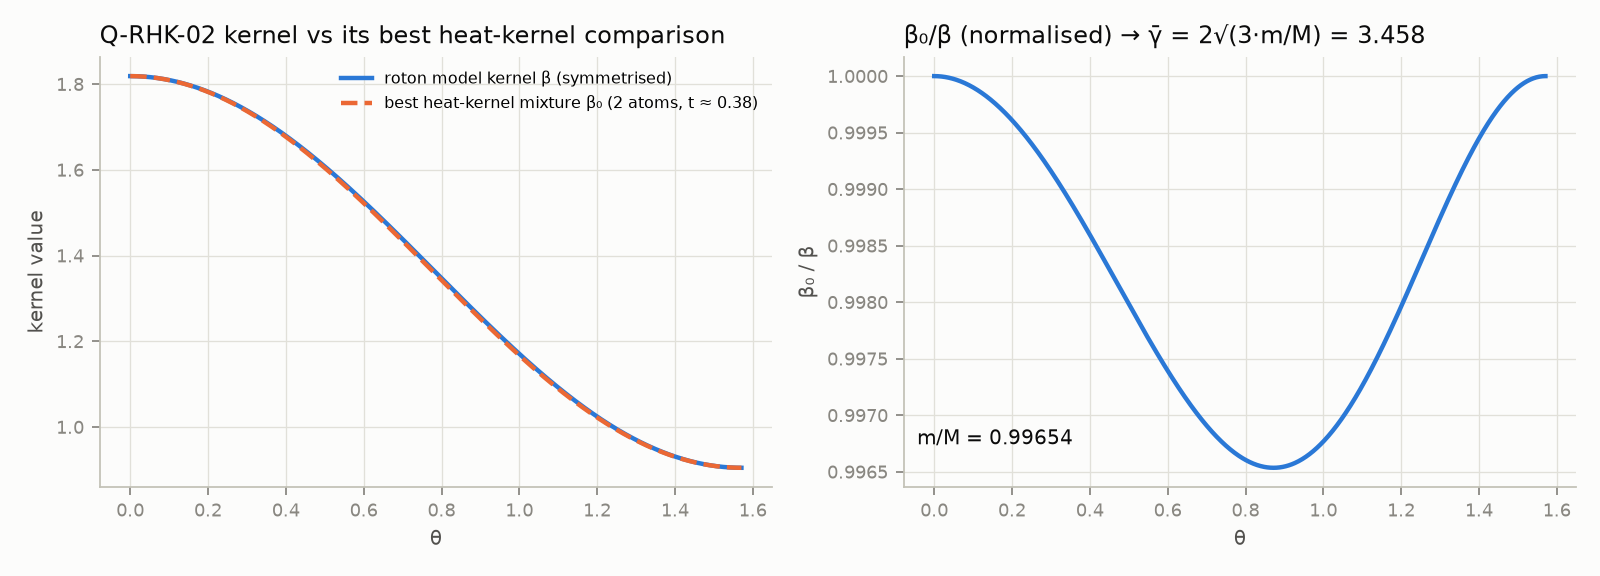
\includegraphics[width=\textwidth]{figures/theorem_22_6/e3_roton_theorem_22_6.png}
\caption{The Q-RHK-02 model kernel and its best heat-kernel comparison (left); their ratio,
$m/M=0.99654$ (right).}
\label{fig:e3}
\end{figure}

%---------------------------------------------------------------------------
\section{Machine-checked kinematics on neutron data}
\label{sec:neutron}
%---------------------------------------------------------------------------

The companion project formalises kinematic identities used in the analysis of neutron scattering
on superfluid $^4$He~\cite{godfrin2021,godfrin2022}. We test them on the dispersion curve
Godfrin \emph{et al.} published with~\cite{godfrin2021}: ILL IN5 data at seven pressures from $0$
to $24.08$~bar, with per-point uncertainties, released as arXiv ancillary files. The files are
fetched and checked by SHA-256, and are not redistributed. The fit reproduces the published sound
velocity ($1.5685$ against $1.5679$~meV\,\AA) and roton gap ($0.7417$ against $0.7445$~meV).

\begin{itemize}
  \item \emph{Maxon versus the roton-pair threshold.} The maxon lies below $2\Delta$ up to
        $10$~bar ($-0.119\pm0.001$~meV) and above it at $24.08$~bar ($+0.0106\pm0.0005$~meV,
        about $21\sigma$), as reported in~\cite{beauvois2018}. A proved lemma states that every
        time-of-flight energy scales with the incident energy, so no proportional recalibration
        can reverse this comparison.
  \item \emph{Top of the measured range.} At saturated vapour pressure the tabulated energy
        at $3.60$~\AA$^{-1}$ ($1.554$~meV) exceeds $2\Delta=1.483$~meV, as the formalisation's
        documentation asserts.
  \item \emph{Three-phonon decay.} It is open if and only if the small-$k$ dispersion curves
        upwards (a proved equivalence). At saturated vapour pressure a fit on
        $Q\le0.15$~\AA$^{-1}$ gives upward curvature at $3.8\sigma$, consistent with the
        published series. The sign change reported near $18$--$20$~bar cannot be decided from
        these files, which start at $Q=0.15$~\AA$^{-1}$ for $P>0$. Our first version of this
        test asserted it anyway; the test was redesigned and the change recorded.
\end{itemize}

%---------------------------------------------------------------------------
\section{Verification and validation}
\label{sec:vv}
%---------------------------------------------------------------------------

We distinguish three levels of evidence and label every claim in this paper by
which level supports it.

\paragraph{Level 1: exact symbolic computation.} The kernel coefficients,
Pad\'e approximants, dispersion polynomials, roots and minimal polynomials are
exact over $\mathbb{Q}$ or $\overline{\mathbb{Q}}$. Forty-nine tests cover these and the
analytic anchors of Sections~\ref{sec:realhe3}--\ref{sec:thm226},
including the two adversarial ones described in Section~\ref{sec:engine}: the
kernel is re-derived from its closed form rather than compared with a table, and
float input is required to raise.

\paragraph{Level 2: independent numerical validation.}
\code{verification/validate\_zero\_sound.py} checks the exact roots against
$60$-digit root-finding and against the asymptotic
law~\eqref{eq:threshold}, and asserts the proved bracket~\eqref{eq:bracket} at every
reference root. It asserts the strong-coupling cases and reports the others, exiting non-zero
only if a regime it claims to have solved degrades. Further scripts, all run in continuous
integration, check the following:
\begin{itemize}
  \item the real-$^3$He analysis of Section~\ref{sec:realhe3};
  \item the neutron-data tests of Section~\ref{sec:neutron};
  \item the reproduction of Section~\ref{sec:thm226};
  \item Fisher-information and entropy monotonicity on the exact Bobylev--Krook--Wu
        solution~\cite{krookwu1976} of the homogeneous Boltzmann equation for Maxwell
        molecules. Mass is conserved exactly, the Maxwellian limit $I=3$ is recovered exactly,
        and both functionals decrease monotonically.
\end{itemize}

\paragraph{Level 3: proof assistant.} The Lean~4 library
\code{AgoraPhysics.Protocols} compiles against mathlib at the pinned revision
\code{ec6e08b4}, and every theorem is accompanied by \code{\#print axioms}. The
scope of that evidence is worth stating plainly.
\code{Protocols.lean} certifies identities such as the $[1/1]$ order condition
$a_2 + q_1 a_1 = 0$ and the fact that $u=10/37$ is a root of $Q - \tfrac{93}{10}P$.
\code{ZeroSoundBracket.lean} and \code{PhaseMixingLink.lean} certify real-analysis statements
about the Landau zero-sound relation and about free transport. None of them certifies anything
about real $^3$He or $^4$He: that connection is made, where it is made, by the data-driven checks
of Level~2. Two theorems in the file are labelled vacuous in the source itself: one
proves $2\cdot 2 = 4$ after unfolding a definition, and one has its hypothesis
as its conclusion. They are retained, labelled, as a record.

%---------------------------------------------------------------------------
\section{Limitations, negative results and retractions}
\label{sec:limits}
%---------------------------------------------------------------------------

\subsection{A capability the method does not have}

The central negative result of this paper concerns the weak-coupling regime.
The kernel~\eqref{eq:chi} has a logarithmic branch point at $s=1$, that is at
$u=1$, which is the edge of the particle--hole continuum. A Pad\'e approximant
constructed from the expansion about $u=0$ represents this branch point by a
finite set of poles, and for small $\Fzs$ the dispersion
polynomial~\eqref{eq:disppoly} then has no root in $(0,1)$ at all: at $M=1$,
Eq.~\eqref{eq:rootformula} gives $u>1$ as soon as $\Fzs < 6/5$. Higher orders do
not repair this, as Table~\ref{tab:conv} shows for $\Fzs \in \{1/10,\,1/2\}$.

The consequence is a retraction of a capability. The protocol registry of this
project previously described tracking ``the velocity ratio drop
$v_{zs}\le v_F$ into the Landau Damping continuum'' by rational Pad\'e
approximants. That is not attainable by this construction, and no
implementation of it ever existed in the repository. The physically correct
statement is that the mode approaches the continuum edge exponentially,
Eq.~\eqref{eq:threshold}, and is exponentially inaccessible to a
finite-order rational approximant built at the origin. The engine now reports
\code{root\_found: false} with a reason in these cases, and a test asserts that
it continues to do so, precisely so that a future change cannot quietly return
a spurious root.

\subsection{Withdrawn claims of earlier versions}

For the record, and because several of these claims are still reachable in the
repository's history and in earlier documents:

\begin{enumerate}
  \item \textbf{The QVE-02 ``echo''} is the Taylor series of
        $\mathrm{Si}(t)^{2}/2$, not a plasma echo (Section~\ref{sec:qve02}).
  \item \textbf{A stored artefact labelled ``True 1D1V Vlasov-Poisson phase
        space simulation''}, with floating-point fields, was never produced by
        any code in this repository. No such solver exists here.
  \item \textbf{$L_*=4$} is definitional (Section~\ref{sec:results}).
  \item \textbf{The ``Theorem 22.6'' attribution} has been checked against the
        source and found mismatched: the paper and theorem are real, but its
        bound is a different, multiplicative object, not the additive formula
        the code computes.
  \item \textbf{Three mutually inconsistent coefficient tables} once coexisted
        for the ``Lindhard'' kernel: $1/3,\,19/45$ in Lean, $2/3,\,2/15$ in
        Python, and $1/(2k+1)$ in the prose. The resolution is that
        $1/(2k+1)$ is correct for the zero-sound kernel~\eqref{eq:ak}, the
        $2/(4k^{2}-1)$ sequence belongs to the different function
        Eq.~\eqref{eq:g}, and $19/45$ corresponded to neither and has been
        removed.
  \item \textbf{``No open dataset exists''} for the roton regime was an earlier conclusion of
        this project's data search. It was wrong: the dispersion data of~\cite{godfrin2021}
        were published openly as arXiv ancillary files, and the search had not looked there.
  \item \textbf{An automated audit of this repository} reported several of these
        repairs as complete before they were. In particular it stated that the
        coefficient tables had been unified across Python and Lean while the
        Lean file was untouched, and that the RPA integration was complete while
        the code was passing a polynomial into a routine expecting a list of
        Taylor coefficients, so that the ``poles'' it produced carried no
        information. Both are recorded in \code{RETRACTIONS.md}.
\end{enumerate}

Item 7 is the reason this section exists in this form. An automated pass that
writes its own audit report is capable of producing a confident, well-formatted
account of work it did not do, which is the first failure mode of
Section~\ref{sec:intro} applied to the act of auditing. The defence is not
more prose; it is the executable checks of Section~\ref{sec:vv}, which fail
when a claim is false.

\subsection{Other limitations}

Contact with measurement is indirect and limited. The data are author-processed tables, not raw
counts; raw ILL data remain to be requested. The angular kernel of Q-RHK-02 is a model, not a fit,
and no available dataset constrains it. The real-parameter zero-sound analysis uses two Landau
parameters and neglects $F_2^s$ and higher, finite temperature and collisions. Its absolute
velocities at the lowest pressures inherit the uncertainty of the source compressibility. The
$d=4$ evidence of Section~\ref{sec:thm226} is numerical and conditional on Theorem~22.6 holding
as stated.

%---------------------------------------------------------------------------
\section{Reproducibility}
%---------------------------------------------------------------------------

All results are produced by the following commands from the repository root. Python
dependencies are pinned in \code{requirements.txt} (\code{sympy}, \code{mpmath}, \code{numpy},
\code{scipy}, \code{matplotlib}, \code{pytest}); \code{poppler-utils} provides \code{pdftotext}.

\begin{verbatim}
  pip install -r requirements.txt
  python3 simulations/qv_01_zero_sound.py            # exact QV-01 derivation
  python3 -m pytest tests/ -q                        # 49 tests
  python3 verification/validate_zero_sound.py        # Tables 2-3, bracket (3.4)
  python3 verification/he3_landau/extract_table_ix.py      # real 3He parameters
  python3 verification/he3_landau/zero_sound_real_he3.py   # Table 4
  python3 verification/helium_kinematics_data.py     # Section 5
  python3 verification/theorem_22_6/reproduce.py     # Section 4 (Python)
  (cd verification/theorem_22_6/rust && cargo run --release)   # (Rust)
  verification/theorem_22_6/run.sh                   # (authors' Julia code)
  cd lean4_formalization && lake exe cache get && lake build   # proofs
\end{verbatim}

The experiments of Section~\ref{sec:thm226}, with their run times, are listed in
\code{verification/theorem\_22\_6/EXPERIMENTS.md}; \code{verification/THEORY\_EXPERIMENT\_LINKS.md}
maps each theorem to the experiment that tests it.

The Lean toolchain is \code{leanprover/lean4:v4.31.0} with mathlib pinned at
\code{ec6e08b4dfb4\-14460f0ee7\-b4ce9678e7\-e04fb584}. Note that
\code{lake exe cache get} is required: compiling mathlib from source takes hours,
and the build that produced the evidence reported here initially failed because
an interrupted clone left the dependency incomplete.

%---------------------------------------------------------------------------
\section{Conclusion}
%---------------------------------------------------------------------------

An exact-rational pipeline can deliver collective-mode velocities as algebraic
numbers with proof-assistant-ready certificates, and at realistic Fermi-liquid
coupling it does so accurately: $6.8\times10^{-10}$ relative agreement with the
transcendental dispersion relation at $\Fzs = 93/10$, improving geometrically
with approximant order. The same analysis shows the method has a hard boundary:
the weak-coupling mode sits exponentially close to a branch point and is
unreachable by rational approximants built at the origin, which retires a
capability this project previously advertised.

Contact with real parameters sharpened this picture rather than confirming it. The
one-parameter model, accurate as mathematics, is wrong as physics for $^3$He: it puts zero
sound below first sound, and the second Landau parameter restores the observed ordering, still
within the exact framework. The threshold law is now a theorem, and the numerics show it is
sharp. Re-examining the numerics behind a published theorem found them sound and slightly
conservative. It also produced evidence that the one case the author left open is covered, which
is offered to the author to check.

The methodological lesson is narrower than the physics but likely more durable.
Every claim in this paper that survived did so because something executable
would fail if it were false: a kernel re-derived from its closed form rather
than compared against a table, a float parameter that raises instead of being
silently rationalised, a validation gate that asserts only the regime it can
actually solve, and an axiom audit rather than a grep for \code{sorry}. The
claims that did not survive, catalogued in Section~\ref{sec:limits}, were
uniformly the ones supported by prose alone, including prose written by an
automated audit about its own work.

%---------------------------------------------------------------------------
\begin{thebibliography}{99}

\bibitem{villani2025}
C.~Villani,
\emph{Fisher Information in Kinetic Theory},
arXiv:2501.00925 (2025).
Lecture notes; Section~22, Theorem~22.6 and Remarks~22.7--22.8 are the subject of
Section~\ref{sec:thm226}. The earlier attribution of Eq.~\eqref{eq:gamma} to Theorem~22.6 was
checked and found mismatched.

\bibitem{godfrin2022}
H.~Godfrin and E.~Krotscheck,
\emph{The Dynamics of Quantum Fluids},
arXiv:2206.06039 (2022).
Cited as a review of $^4$He and $^3$He dynamics. Neither author has reviewed or
endorsed this code.

\bibitem{isv2024}
C.~Imbert, L.~Silvestre and C.~Villani,
\emph{On the monotonicity of the Fisher information for the Boltzmann equation},
arXiv:2409.01183 (2024).

\bibitem{silvestre2024}
L.~Silvestre, \emph{Collision kernels} (Julia code),
\url{https://github.com/luissilvestre/collisionkernel}, commit \code{01a9d44} (2024).

\bibitem{godfrin2021}
H.~Godfrin, K.~Beauvois, A.~Sultan, E.~Krotscheck, J.~Dawidowski, B.~F\aa k and J.~Ollivier,
\emph{Dispersion relation of Landau elementary excitations and thermodynamic properties of
superfluid $^4$He}, Phys.\ Rev.\ B \textbf{103}, 104516 (2021), arXiv:2012.09067, with
ancillary data files.

\bibitem{beauvois2018}
K.~Beauvois, J.~Dawidowski, B.~F\aa k, H.~Godfrin, E.~Krotscheck, J.~Ollivier and A.~Sultan,
\emph{Microscopic dynamics of superfluid $^4$He: a comprehensive study by inelastic neutron
scattering}, Phys.\ Rev.\ B \textbf{97}, 184520 (2018).

\bibitem{kollar2000}
M.~Kollar and D.~Vollhardt,
\emph{Thermodynamically consistent equilibrium properties of normal-liquid Helium-3},
Phys.\ Rev.\ B \textbf{61}, 15347 (2000), arXiv:cond-mat/9906222.

\bibitem{greywall1983}
D.~Greywall, Phys.\ Rev.\ B \textbf{27}, 2747 (1983). The specific-heat data from which the
tables of~\cite{kollar2000} are derived (their ref.~16).

\bibitem{krookwu1976}
M.~Krook and T.~T.~Wu, \emph{Formation of Maxwellian tails},
Phys.\ Rev.\ Lett.\ \textbf{36}, 1107 (1976).

\bibitem{pinesnozieres}
D.~Pines and P.~Nozi\`eres,
\emph{The Theory of Quantum Liquids}, Vol.~I,
W.~A.~Benjamin, New York (1966).
Standard treatment of zero sound and of the dispersion relation
\eqref{eq:disp}.

\bibitem{bakergravesmorris}
G.~A.~Baker~Jr.\ and P.~Graves-Morris,
\emph{Pad\'e Approximants}, 2nd ed.,
Cambridge University Press (1996).

\bibitem{mathlib}
The mathlib Community,
\emph{The Lean Mathematical Library},
CPP 2020, pinned revision \code{ec6e08b4}.

\end{thebibliography}

\end{document}
